\chapter{Úvod}
%\addcontentsline{toc}{chapter}{Úvod}

Strategické hry jsou žánrem, ve kterém hráči využívají svých mentálních schopností, především taktického a strategického myšlení, pro dosažení cíle. To je jedním z důvodů, proč je tento druh her oblíben mezi studenty naší fakulty. Naše práce se zaměří na ulehčení tvorby konkrétního poddruhu strategických her, a to \emph{Real-time strategy} (RTS) her. K tomuto účelu bude vytvořena platforma rozšiřující herní engine UrhoSharp pro tvorbu RTS her. Oproti předešlým pracím, které se většinou zabývaly 2D RTS hrami, se my pokusíme vytvořit platformu umožňující tvorbu 3D RTS her.

\section{RTS hry}
Real-time strategy hry, v překladu strategické hry probíhající v reálném čase, jsou poddruhem strategických her ve kterém se změny stavu odehrávají v přímé závislosti na změně času v reálném světě. Tato vlastnost je odlišuje od tahových strategických her, ve~kterých má hráč neomezenou dobu na přemýšlení o svém tahu, což mu umožňuje vymyslet optimální strategii. Reakce v reálném čase jsou náročnější jak pro hráče, který je často nucen použít suboptimální strategii, tak pro hru samotnou, která musí provádět výpočet dalšího stavu v omezeném čase a a s omezeným výkonem, o který bojuje s vykreslováním hry. Stejně tak umělá inteligence hráčů musí reagovat na aktivity zbylých hráčů s omezeným časem a výkonem, což limituje množství dat a složitost výpočtu, které může umělá inteligence použít. Z tohoto důvodu je vývoj RTS her složitým procesem, spojujícím mnoho oborů. 

Již od svého vzniku na konci osmdesátých let a začátku devadesátých let minulého století \todo{jiný slovo než obsahovaly} obsahovaly RTS hry několik konceptů, které lze nalézt v drtivé většině her tohoto žánru i dnes. 

Těmito koncepty jsou:
\begin{itemize}
	\item Výroba a ovládání jednotek s cílem ovládnutí části mapy a zničení nepřátelských jednotek a budov
	\item Stavba budov pro umožnění stavby nových druhů budov, jednotek či získání surovin
	\item Získávání surovin pro stavbu jednotek a budov
	\item Výzkum nových technologií
\end{itemize}

Základním stavebním kamenem RTS her je pečlivé vyvážení kombinace strategie/macromanagementu a taktiky/micromanagementu. Tyto pojmy bývají často špatně chápány a někdy zaměňovány, pokusíme se je proto konkrétně definovat. Strategií míníme \todo{citace} rozhodnutí týkající se globálního průběhu hry. Taktika \todo{citace} naopak zahrnuje konkrétní pozice konkrétních jednotek, jejich pohyb po mapě a spolupráci v jedné bitvě.  

Mezi strategická rozhodnutí v RTS hrách patří kupříkladu které budovy hráč postaví, v jakém pořadí dané budovy postaví, které suroviny bude produkovat, které suroviny vynechá, které jednotky bude rekrutovat a které vynechá. \todo{mozna graf nasledujiciho, jak se ovlivnujou} Tato 3 rozhodnutí jsou úzce propojena, protože výběr surovin určuje budovy, které bude hráč schopen postavit a typy jednotek, které bude moci zrekrutovat. Stejně tak výběr budov určuje suroviny, které hráč může produkovat a typy jednotek, které může zrekrutovat. \todo{pojem ekonomie}. 

Taktika/micromanagement je v RTS hrách reprezentován ovládáním jednotek, jejich přesné pozice, pohybu, směru útoku, používání schopností atd. Micromanagement lze ale vidět i v ekonomické stránce hry, kdy hráč 

Nejlepším příkladem pro rozlišení pojmu strategie a taktiky je série her Total War, které kombinuje mód tahové strategie s módem real-time tactics (RTT). V jedné části hry hráč přebírá kontrolu nad celým svým národem, rozhoduje, které budovy budou ve kterých městech postaveny, které jednotky budou rekrutovány a kde budou které armády umístěny. V druhé části, při souboji nepřátelských armád, hráč přebírá kontrolu nad konkrétní armádou a ovládá jednotlivé bataliony, jejich umístění, pohyb a útoky v reálném čase.

Tento příklad nám také ukazuje sousední žánry her na spektru důležitosti strategie a taktiky. Na jedné straně máme tahové strategie, které oproti RTS minimalizují důležitost micromanagementu a soustředí se především na globální strategii. Tahové strategie se vyvinuly ze stolních her, od kterých přebraly velkou část svých herních mechanik. \cite{https://web.archive.org/web/20081201113349/http://archive.gamespy.com/articles/february02/strat04/index.shtm}. Na druhé straně spektra máme RTT a turn-based tactics hry, které se zbavují strategických prvků v podobě surovin a budov, výměnou za větší taktické možnosti a detailnější ovládání jednotek. Příkladem čistě RTT her může být série Blitzkrieg \todo{odkaz nebo citace}. Nejznámějším zástupcem turn-based tactics her je série her X-COM.  

Hranice mezi RTT a RTS není přesně definována, jedná se spíše o plynulý přechod mezi těmito dvěma žánry. Dnešní RTS hry bývají často kritizovány pro zvyšující se důležitost taktiky na úkor strategie, což je posouvá stále blíže k žánru RTT. Tento posun také mění schopnosti potřebné pro hraní těchto her. Postupný přechod k micromanagementu dává velkou výhodu hráčům s rychlejšími reakcemi místo hráčů schopných strategického myšlení.

Jako příklad RTS můžeme vzít hru \emph{Dune II}, která je považována za první hru obsahující všechny prvky RTS.\cite{} Samotný název "real-time strategy", poprvé použitý při propagaci této hry, je připisován prezidentu a spoluzakladateli Westwood Studios, \emph{Brettu Sperrymu}. Toto studio následně využilo zkušenosti získané při tvorbě Dune II pro vývoj jedné z nejznámějších sérií RTS her, Command \& Conquer.


\todo{popsat Dune II}

Hlavní inspirací pro tvorbu platformy, a tím i pro typ her, které bude platforma nejjednodušeji podporovat, byla hra Stronghold. Na této hře, vydané v roce 2002, ukážeme blíže základní principy RTS her.

\subsection{Jednotky}
Jednotky jsou základním nástrojem hráče pro boj s nepřítelem. Pohybem po mapě, poškozováním ostatních jednotek a ničením budov jednotky umožňují hráči vést souboj s protivníkem, získat strategickou výhodu a následně vyhrát hru. 

Hlavním odlišujícím prvkem od budov je možnost pohybu. Tento pohyb je nejčastěji řízen hráčem, ať už na úrovni příkazů jednotlivým jednotkám, tak na úrovni slučování jednotek do skupin a ovládání těchto skupin. Ve velké části RTS her jsou jednotky schopny do určité míry autonomního rozhodování bez zásahu hráče, od střelby na cíl, který se ocitne v jejich dostřelu, po vyhledání krytu, pokud jsou pod palbou. Dobrým příkladem jednotek s vysokou autonomií je série Company of Heroes, kde jednotky automaticky vyhledávají krytí, rozutečou se, pokud jsou pod palbou dělostřelectva, a v případě příliš velkých ztrát utečou z boje. 

Tato autonomie má ale svou cenu, a to v nepředvídatelnosti chování jednotek. Při jednoduché umělé inteligenci jednotek je hráč schopen předvídat jejich chování a využít ho pro svůj prospěch. Naopak při složité umělé inteligenci, jako právě v případě Company of Heroes, je hráč často nucen provést více pokusů při vydávání rozkazu , protože není schopen jednoduše odhadnout chování jednotky. Tato skutečnost činí hry často realističtější, protože simuluje chování reálných vojáků, kteří rozkaz interpretují a implementují podle svého, není ale vhodná pro souboje více hráčů, a už vůbec né více hráčů na profesionální úrovni.

Jako příklad jednoduché umělé inteligence jednotek můžeme vzít hry Starcraft a Warcraft od společnosti Blizzard. Zde se jednotky chovají velice předvídatelně, splňují přesně hráčovi rozkazy a nedělají nic navíc, což umožnilo hře Starcraft II vytořit jednu z prvních masivních e-sport scén na světě. \cite{http://www.gamasutra.com/php-bin/news_index.php?story=18326}

Pro RTS hry je možnost produkce nových jednotek jednou z definujících vlastností. Existuje několik systémů produkce jednotek, úzce svázaných se systémem surovin v dané hře. \todo{see Suroviny} Od kontinuální produkce, kde hráč zvolí produkované jednotky a suroviny jsou spotřebovávány v průběhu produkce, po diskrétní produkci, kde hráč musí vlastnit všechny suroviny potřebné pro výrobu dané jednotky při začátku produkce a všechny suroviny jsou odečteny v jeden okamžik. Kontinuální systém umožňuje hráči naplánovat produkci armády v předstihu, i když v daném okamžiku nevlastní dostatečné suroviny. Naopak při diskrétní produkci je hráč nucen čekat do chvíle, kdy má všechny suroviny, a až poté může začít s produkcí.

Možnosti produkce jednotek také mění taktické volby hráče. Jednotky nemají hodnotu pouze podle své výkonosti v boji, ale také podle doby a ceny produkce. Hráč je mnohem ochotnější obětovat velké množství levných, rychle obnovitelných jednotek než drahých a vzácných jednotek. Hodnota jednotky také může být pro každého hráče různá, podle jeho aktuální ekonomické situace, dostupnosti surovin a podle strategie zvolené nepřítelem. Čas pro produkci jednotek omezuje rychlost změny strategie v reakci na nepřítelovu strategii.

Poměr ceny produkce jednotek a ceny vyzkoumání nových jednotek je jedním z hlavních faktorů určujících strategické možnosti hráče. Při levých jednotkách a drahém postupu je nejlepší strategií výroba velkého počtu dostupného typu jednotek místo odemykání nových silnějších jednotek. To poté vede k tomu, že ve velké většině her se hráči nikdy nedostanou k vývoji nových jednotek a hra skončí porážkou jednoho z hráčů pomocí starších jednotek. Oproti tomu při velké ceně produkce oproti levnějšímu odemykání nových silnějších typů probíhá hra často bez větší konfrontace hráčů až do vyzkoumání posledního stupně jednotek, po kterém pak hráči mohou dedikovat všechny suroviny pro výrobu.

Počet jednotek je často limitován, jak pro účely vyvážení hry, tak pro omezení zátěže hardwaru. Z hlediska vyvážení síly jednotek umožňuje limit na počet jednotek předejít tzv. "Zergu", kdy hráč vytvoří obrovské množství levných jednotek, které následně převálcují jakýkoli odpor. Z hlediska hardwarové náročnosti je účel limitu vcelku zřejmý, protože každá jednotka zabírá určité množství paměti a výpočetního výkonu.

Hráč často začíná s malým počtem jednotek, jejichž účelem je zamezit tzv. Rush strategii, ve které je cílem vytvořit co nejrychleji co nejvíce levných jednotek a zničit nepřítele ještě před tím, než je schopen začít produkovat své jednotky.

Ve hře Stronghold začíná hráč hru s malým počtem jednotek z výše uvedeného důvodu. Ve hře Stronghold Crusader, s kterou je autor nejvíce seznámen, jsou jednotky dvojího typu. Prvním typem jsou arabské jednotky, produkované v arabských kasárnách, které stojí pouze zlaťáky. Druhým typem jednotek jsou křižácké jednotky, produkované v křižáckých kasárnách, které jsou o řád levnější ve zlaťácích než jejich arabské protějšky, ale navíc stojí zbraně a brnění, které je potřeba vyrábět. Arabské jednotky je bohatý hráč schopný rekrutovat velice rychle, a tím vytvořit velkou armádu ve velice krátkém čase. Křižácké jednotky jsou o něco silnější, ale jejich produkce je omezena výrobou zbraní a brnění, není tedy možné bez předchozí přípravy rychle vytvořit armádu křižáckých jednotek. Toto je jeden z příkladů strategického rozhodnutí, které musí hráč učinit, a to zda bude produkovat ve zlatě levnější, silnější, ale časově a surovinově náročnější křižácké jednotky, nebo se bude soustředit na vydělávání zlata a rychlou produkci slabších arabských jednotek. 

Jednotky mají jako ve většině RTS her určitý počet hit pointů, které s každým obdrženým zraněním ubývají, dokud není jednotka zabita. Poškození je určeno typem jednotky, kde každá jednotka má skrytý modifikátor poškození, které obdrží z různých zdrojů.
\todo{popsat concrete a abstract balancing výše} Toto je příklad abstraktního balancingu.

Počet jednotek je omezen na 1000 pro každého hráče, především pro omezení hardwarové náročnosti. 

\subsection{Budovy}
Budovy slouží mnoha účelům, nejčastěji zajišťují sběr surovin, tvorbu jednotek a často jsou také používány přímo pro boj. Budovy a z nich tvořené základny umožňují hráči v průběhu času zvětšovat svou sílu v podobě nových jednotek, budov a většího množství surovin, a tuto sílu využít k porážce nepřítele. To bývá používáno jako hlavní bod pro odlišení čistě taktických her, kde hráč začíná boj se svou plnou silou, nejčastěji v podobě jednotek, a postupně v boji o tuto sílu přichází bez možnosti jejího doplnění. Mezi taktické hry splňující tuto definici patří například hry ze sérií \cite{Total War}, \cite{X-COM} nebo české série \cite{UFO}.

Ve hře Stronghold je stavba budov implementována vcelku jednoduše. Hráčovi jsou všechny dostupné budovy nabídnuty v menu bez možnosti odemknout v průběhu hry další budovy. Po zvolení z nabídky lze pohybem kurzoru v herním poli vybrat umístění budovy. Pokud má hráč dostatečný počet surovin a terén budově vyhovuje, objeví se po kliknutí tato budova na vybraném místě. Podobně funguje stavba budov i v dalších RTS hrách, jako \cite{Company of Heroes}, \cite{}

\subsection{Suroviny}
Resource management je přítomný ve všech hrách tohoto žánru již od jeho vzniku. Od koření v Dune II, přes zlato a dřevo ve Warcraft 3, po všechny typy surovin ve hře Stronghold, získávání surovin je jednou z hlavních motivací konfliktu v RTS hrách. 

Systémy surovin lze rozdělit podle způsobu získávání a počtu typů surovin.

Podle způsobu získávání můžeme systém surovin rozdělit na
\begin{enumerate}
	\item Aktivní získávání surovin
	\item Pasivní získávání surovin
\end{enumerate}

Při aktivním získávání surovin existuje ovladatelná herní entita, která svým pohybem mezi pozicemi na mapě přináší suroviny. Tento pohyb může být ovládán hráčem, ale nejčastěji dokáže pracovat jednotka samostatně. Příkladem může být Warcraft, kde speciální jednotky získávají dřevo a zlato přenášením z lesů/dolů do hráčovy hlavní budovy.

Při pasivním získávání přibývají suroviny bez akcí entit, pouze díky vlastnictví určité části mapy nebo druhu budovy. Zdroj bývá nekonečný nebo skoro nekonečný, poskytující suroviny do obsazení nebo zničení zdroje.

Každý z těchto stylů podporuje jinou strategii kontroly mapy. 


Při aktivní získávání surovin je celkový zisk nejčastěji omezen počtem jednotek pracujících na dané surovině, což umožňuje hráči bránit pouze několik málo pozic, mezi kterými se tyto jednotky pohybují, čímž umožňuje hráči postavit svoji ekonomiku z velké části bez ohledu na akce nepřítele.

Pasivní získávání surovin naopak nutí hráče obsazovat a kontrolovat mnoho částí mapy, které slouží jako zdroje suroviny, jak pro svoje vlastní potřeby surovin, tak pro odepření daného zdroje nepříteli. Toto vede k velice hektickému průběhu hry, kdy hráč paralelně vede souboj na mnoha frontách pro obsazení co největší části mapy a získání výhody v počtu surovin.

Tyto dva styly systému získávání surovin lze také kombinovat. Získání pasivního zdroje může sloužit pro uvolnění zdrojů dedikovaných pro aktivní získávání surovin, naopak ztráta pasivního zdroje může být nahrazena zvýšením výkonu aktivního zdroje.


Větší počet druhů surovin by měl hráči umožnit strategicky se rozhodnout, které suroviny bude získávat a které bude ignorovat. Toto rozhodnutí následně ovlivní typy jednotek a budov, které hráč bude stavět a tím i celou strategii dané hry. Zde může nastat problém, kdy hra nutí hráče získávat všechny druhy surovin a neumožňuje hráči vybírat si. Tím je ztracena výhoda více surovin a strategie při hraní této hry budou velice podobné strategiím pro hry s jedním druhem surovin.
\subsection{Vývoj technologií}
Volba vyzkoumaných technologií důležitou součástí strategické části RTS her. 

Technologie jsou často uspořádány ve stromové struktuře, kde vyzkoumání technologie v rodičovském uzlu odemyká technologie ve svých synech. Každé větvení představuje možné rozhodnutí hráče, kterou z větví bude dále zkoumat. V některých hrách bývají dokonce větve výlučné, tedy vyzkoumání jedné větve zamkne přístup k vyzkoumání jiné větve.

Vyzkoumání technologie může mít mnoho různých efektů. Nejčastějším efektem bývá odemknutí nového typu jednotek nebo budov. Další možností je změna vlastností již vlastněných jednotek nebo budov. V neposlední řadě pak může vyzkoumání technologie odemknout nové schopnosti nebo kouzla, které hráč může následně použít při taktických soubojích. 

Explicitní strom technologií, přítomný např. ve hrách série Civilisation, se v RTS hrách vyskytuje spíše výjimečně. Nejčastěji je odemykání nových typů jednotek a budov umožněno stavbou určitého typu budovy nebo dosažení určitého stupně vylepšení již existující budovy. Jako příklad můžeme vzít Warcraft 3, kde závislosti budov na stupních vylepšení a existenci jiných budov tvoří strom technologií. 

\begin{figure}[h]
	\caption{Výřez stromu technologií ze hry Civilisation V}
	\centering
	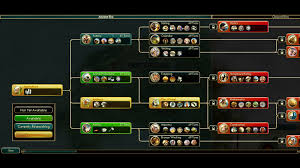
\includegraphics{civ5_tech_tree}
\end{figure}


\begin{figure}[h]
\caption{Budovy a závislosti mezi nimi tvořící obdobu stromu technologií ve hře Warcraft 3}
\centering
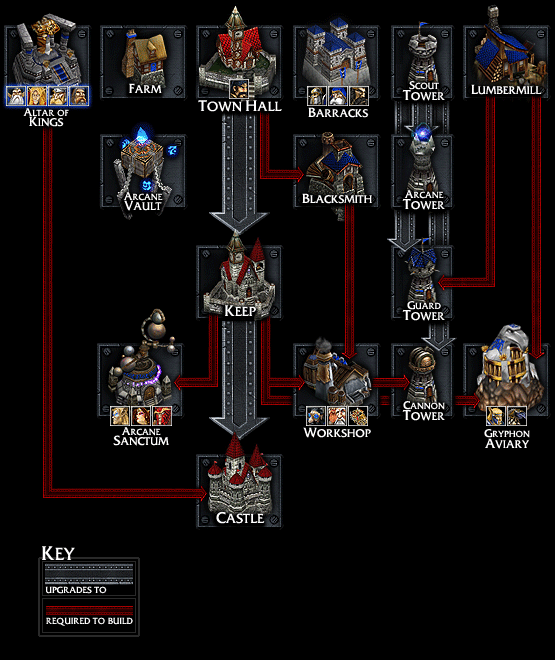
\includegraphics{warcraft_tech_tree}
\end{figure}

Ve hře Stronghold vývoj technologií také není explicitně přítomen, přístup k novým typům jednotek a budov je místo toho znemožněn dostupností surovin a nutností výstavby řetězce pro produkci určitých druhů surovin. 

\section{Požadavky}
Žánr RTS her, jak jsme jej popsaly v předešlé sekci, je pro tvorbu jednoho frameworku podporujícího vývoj všech RTS her příliš rozsáhlý a zahrnuje hry s příliš rozdílnými požadavky na vývoj. Proto jsme se rozhodli v naší práci implementovat framework umožňující vývoj podmnožiny žánru RTS, a to 3D RTS her pro jednoho hráče s mapou rozdělenou na homogenní čtvercové dlaždice. 

Náš framework bude tedy poskytovat prvky společné hrám tohoto druhu, přičemž bude umožňovat vývojáři hry co největší možnosti pro rozšíření poskytovaných prostředků s 
co možná nejmenším omezením na mechaniky her vyvíjených za pomoci našeho frameworku.
 
Hlavním cílem našeho framework je možnost využití .NET Frameworku pro vývoj pluginů, které poté spolu s assety a metadaty vytvoří balíček. Tento balíček poté hráč bude moci přidat do své hry, čímž získá přístup k novým jednotkám, budovám, mapám, typům dlaždic, surovin a oponentů. 

Pro implementaci jsme so rozhodli použít UrhoSharp engine, nad kterým postavíme náš framework a pokusíme se zjednodušit využití tohoto enginu pro tvorbu našeho poddruhu RTS her. 
\begin{enumerate}
	\item Z pohledu tvůrce balíčku bude náš framework sloužit jako knihovna, spouštějící tvůrcovi funkce v reakci na události nastávající ve~hře. Dále bude poskytovat implementaci herní mapy a centrálního registru všech entit, do kterých se logiky jednotek, budov a hráčů budou schopny dotazovat na aktuální stav hry. Pro předejití opakované implementace každým tvůrcem her bude dále poskytovat základní komponenty, umožňující pohyb jednotek po mapě, pohyb projektilů po balistických křivkách a výpočty cílů podle pohybu jednotek, automatickou střelbu na cíle, \todo{popsat všechny DefaultComponenty}. V neposlední řadě bude umožňovat ukládání a zpětné načítání aktuálního stavu hry, spolu s rozhraním pro ukládání a zpětné načítání stavu logiky definované tvůrcem hry. 
	
	Dále framework z pohledu tvůrce balíčku bude sloužit jako spustitelný software, poskytující editor mapy, spolu se základní implementací nástrojů pro její editaci, umožňující změnu výšky jednotlivých rohů dlaždic, dlaždic jako celku nebo i skupin dlaždic. Dále bude umožňovat takto vzniklý hrubý terén zarovnat. Spolu s těmito nástroji pro změnu tvaru terénu bude umožňovat změnu typu na všechny typy dlaždic definované v aktuálně používaném balíčku. Tvůrcům balíčků bude umožněno odebírat tyto základní implementace a přidávat odvozené nebo úplně nové editační nástroje, které pak budou schopni použít při tvorbě map v našem editoru.
	
	Formát uložení hry bude veřejně známý, bude tedy možné vytvářet nezávislé nástroje pro tvorbu a editaci map. 
	\item
	Z pohledu hráče bude framework jako samostatný spustitelný software umožňovat načítání balíčků, editaci map připravených tvůrcem balíčku, vytváření úplně nových map používajících jednotky, budovy, oponenty a typy dlaždic poskytnuté tvůrcem balíčku a následné spuštění všech takto získaných map. V průběhu hry potom bude umožňovat uložení aktuálního stavu hry a následné načtení tohoto stavu.
\end{enumerate}




Pro ukázku bude vytvořena jednoduchá hra, demonstrující možnosti našeho frameworku. \todo{Popsat hru}

\section{Cíle práce}
Cílem této práce je vytvořit framework pro vývoj 3D RTS her pro jednoho hráče, umožňující vývojářům vytvářet hry jako separátně 
distribuované balíčky, které bude poté koncový uživatel schopen připojit do našeho frameworku nainstalovaném na uživatelově počítači.

Při tvorbě balíčků bude umožněno tvůrci použít .NET Framework pro vytvoření Umělé inteligence jednotek, budov a AI hráčů, dále pro přidání nástrojů do editoru map a \todo{ Nespecifické } kontrolu průběhu hry.

Požadované vlastnosti frameworku:
\begin{enumerate}
	\item Vlastnosti pro tvůrce balíčků:
		\begin{enumerate}
			\item Framework musí umožňovat přidávání balíčků za běhu, obsahujících nové typy jednotek, budov,  dlaždic, projektilů a hráčů spolu s jejich modely, texturami a AI.
			\item Framework musí umožňovat použití přidaných balíčků pro tvorbu map a uložení vytvořených map do balíčku použitého pro jejich vytvoření
			\item Editor map musí být rozšiřitelný pomocí pluginů z balíčku.
			\item Herní user interface musí umožňovat rozšiřitelnost pro tlačítka, okna a další grafické prvky přidávané tvůrcem.
		\end{enumerate}

	\item Vlastnosti pro koncového hráče:
		\begin{enumerate}
			\item User interface pro stolní počítače, umožňující vybírání balíčků, map a oponentů, dále načítání a ukládání her, a nastavování zobrazení hry.
			\item Herní user interface musí obsahovat minimapu, poskytující hráči přehled o větší části mapy než kterou vidí vlastní kamerou.
			\item Ovládání kamery umožňující klasický top-down pohled, volné poletování kamery po mapě a následování jednotky
			\item Ukládání a načítání hry
		\end{enumerate}
\end{enumerate}
